\documentclass[UTF8]{article}
\usepackage{ctex}
\usepackage{ulem}
\usepackage{amssymb}
\usepackage{amsmath}
\usepackage{graphicx}
\newtheorem{thm}{定义}[section]
\newtheorem{notation}[thm]{记号}
\newtheorem{lemma}[thm]{引理}

\makeatletter
\newcommand{\rmnum}[1]{\romannumeral #1}
\newcommand{\Rmnum}[1]{\expandafter\@slowromancap\romannumeral #1@}
\makeatother

\title{$\lambda{\rm C}$中逻辑概念的编码\\The encoding of logical notions in $\lambda{\rm C}$\\[2ex]\begin{large}读书笔记\end{large}}
\author{许博}
\date{}

\begin{document}
\maketitle
	\section{疑问}
	\noindent
	1. P142. 析取的表示$A\lor B\equiv\Pi C:*.(A\rightarrow C)\rightarrow(B\rightarrow C)\rightarrow C$,对它的解释为:\textit{If A implies C and also B implies C, then C holds on its own}。为什么这里的$A$和$B$是或的关系?是否因为其为真时满足($A\lor B$)为真,算是强行解释吗?

	\section{类型理论中的谬论(absurdity)与否定(negation)}
	\noindent
	在章节 5.4 中,通过编码蕴含式$A\Rightarrow B$为函数类型$A\rightarrow B$,模拟蕴含式的行为,包括它的导入和消解规则。因为$\lambda{\rm P}$是$\lambda{\rm C}$的一部分,所以$\lambda{\rm C}$中同样拥有最小谓词逻辑。
	
		本章将处理更多的接词(connective),比如否定($\neg$),合取($\land$)和析取($\lor$)。这些在$\lambda{\rm P}$中不能表示,但在$\lambda{\rm C}$中存在非常优雅的方式去编码这些概念。
		
		将否定$\neg A$看作蕴含式$A\Rightarrow \bot$,其中$\bot$是“谬论(absurdity)”,也可以称为“矛盾(contradiction)”。因此$\neg A$被解释为“$A$蕴含了谬论”。为了这个目标,我们需要谬论的编码:\\
		
	\noindent
	\textit{\Rmnum{1}. 谬论,Absurdity}\\
	命题“谬论”或$\bot$的一个独特的性质是:如果$\bot$为真,则每一个命题都为真。
	
		每一个命题都为真,则存在一个接收任意一个命题$\alpha$然后返回$\alpha$的一个成员的函数,而这个函数的类型为$\Pi\alpha:*.\alpha$。因此“如果$\bot$为真,则每一个命题都为真”可以表述为“如果存在$M:\bot$,则存在$f:\Pi\alpha:*.\alpha$”。因此,在类型理论中,定义$\bot$为$\Pi\alpha:*.\alpha$。
		
		$\bot$-消解($\bot$-elimination)规则:
		
		($\bot$-elim) $\cfrac{\bot}{A}$
		
		因为$\bot\equiv\Pi\alpha:*.\alpha$,则$s_1=\square$且$s_2=*$,所以$\bot$存在于$\lambda{2}$中,且$\bot:*$。\\
		
	\noindent
	\textit{\Rmnum{2}. 否定,Negation}\\
	定义:$\neg A\equiv A\rightarrow\bot$。
	
		$A\rightarrow\bot$是$\Pi x:A.\bot$的简写,其中$A:*$且$\bot:*$,所以$(s_1,s_2)=(*,*)$。但因为$\bot$存在,至少$\lambda{2}$才能够表示否定。
		
		$\bot$-导入($\bot$-introduction)规则:
		
		($\bot$-intro) $\cfrac{A\ \ \ \neg A}{\bot}$
		
		或:
		
		($\bot$-intro) $\cfrac{A\ \ \ A\Rightarrow\bot}{\bot}$
		
		而($\neg$-intro)和($\neg$-elim)规则可以以($\Rightarrow$-intro)和($\Rightarrow$-elim)规则替换,前者为后者的特殊情况。
		
		需要注意的是,尽管($\bot$-intro)和($\neg$-elim)都是($\Rightarrow$-elim)的特殊情况,但两者具有不同的目的,前者是为了获得$\bot$,而后者则告诉了我们如何使用一个否定$\neg A$。
		
	\section{类型理论中的合取和析取}
	\noindent
	\textit{\Rmnum{1}.合取,Conjunction}\\
	合取$A\land B$为真当且仅当$A$和$B$都为真。在$\lambda{2}$中,合取的表示为:
	
		$A\land B\equiv\Pi C:*.(A\rightarrow B\rightarrow C)\rightarrow C$
		
		这是一个合取的所谓“二阶”编码,比如$A\land B\equiv\neg(A\rightarrow\neg B)$的一阶编码更为通用,因为后者只在经典逻辑中有效。
		
		$\Pi C:*.(A\rightarrow B\rightarrow C)\rightarrow C$可以读作:\textit{对于所有的C,(A蕴含(B蕴含C))蕴含C}。若将$A,B,C$都看作是命题,则可以解释为:\textit{对于所有命题C,如果A和B共同蕴含C,则C取决于自身}。条件“如果A和B共同蕴含C”也即“A和B都为真”是多余的,而为了使条件成立,A和B必须为真。这里我认为,$C$ holds on its own 意为 $C\rightarrow C$,也即第二个$C$由第一个$C$蕴含,而$C\rightarrow C$恒为真,所以条件是多余的,但条件需要满足(条件满足是命题为真的必要条件),所以A和B都需要为真。
		
		$\Pi C:*.(A\rightarrow B\rightarrow C)\rightarrow C$被称为二阶是因为它是在命题上的泛化,而命题是二阶对象。
		
		$\land$在自然演绎中的规则以及在类型理论中二阶编码的规则:
		
		($\land$-intro) $\cfrac{A\ \ \ B}{A\land B}$
		
		($\land$-elim-left) $\cfrac{A\land B}{A}$
		
		($\land$-elim-right) $\cfrac{A\land B}{B}$
		
		($\land$-intro-sec) $\cfrac{A\ \ \ B}{\Pi C:*.(A\rightarrow B\rightarrow C)\rightarrow C}$ 
		
		($\land$-elim-left-sec) $\cfrac{\Pi C:*.(A\rightarrow B\rightarrow C)\rightarrow C}{A}$
		
		($\land$-elim-right-sec) $\cfrac{\Pi C:*.(A\rightarrow B\rightarrow C)\rightarrow C}{B}$ \\
		
	\noindent
	\textit{\Rmnum{2}. 析取,Disjunction}\\
	析取$A\lor B$的二阶编码:
	
		$A\lor B\equiv\Pi C:*.(A\rightarrow C)\rightarrow(B\rightarrow C)\rightarrow C$
		
		与合取的讨论相似,右边的表达式可以读作:\textit{对于所有C,(A$\rightarrow$C蕴含(B$\rightarrow$C蕴含C))}。将$A,B,C$看作命题,则可以解释为:\textit{对于所有的命题C,如果A蕴含C并且B也蕴含C,则C取决于自身},在逻辑上等价于:\textit{如果(A或B)蕴含C,则C成立(hold)}。(这里的逻辑等价可能是指真值表相同?)。条件是多余的,所以$A$或$B$必须成立。
		
		$\lor$在自然演绎中的规则:
		
		($\lor$-intro-left) $\cfrac{A}{A\lor B}$
		
		($\lor$-intro-right) $\cfrac{B}{A\lor B}$
		
		($\lor$-elim) $\cfrac{A\lor B\ \ \ A\Rightarrow C\ \ \ B\Rightarrow C}{C}$
		
		$\lor$在类型理论中二阶编码的规则:
		
		($\lor$-intro-left-sec) $\cfrac{A}{\Pi C:*.(A\rightarrow C)\rightarrow(B\rightarrow C)\rightarrow C}$
		
		($\lor$-intro-right-sec) $\cfrac{B}{\Pi C:*.(A\rightarrow C)\rightarrow(B\rightarrow C)\rightarrow C}$
		
		($\lor$-elim-sec) $\cfrac{\Pi D:*.(A\rightarrow D)\rightarrow(B\rightarrow D)\rightarrow D\ \ \ A\rightarrow C\ \ \ B\rightarrow C}{C}$
		
		至此,我们已经定义了类型理论中否定,合取以及析取的变体:
		
		$\neg A\equiv A\rightarrow\bot$
		
		$A\land B\equiv\Pi C:*.(A\rightarrow B\rightarrow C)\rightarrow C$
		
		$A\lor B\equiv\Pi C:*.(A\rightarrow C)\rightarrow(B\rightarrow C)\rightarrow C$
		
		但是在这三者中,$A,B$都是自由变量,因此引入单个连词使得可以用于更“抽象”的表达式:
		
		$\neg\equiv\lambda\alpha:*.(\alpha\rightarrow\bot)$
		
		$\land\equiv\lambda\alpha:*.\lambda\beta:*.\Pi\gamma:*.(\alpha\rightarrow\beta\rightarrow\gamma)\rightarrow\gamma$
		
		$\lor\equiv\lambda\alpha:*.\lambda\beta:*.\Pi\gamma:*.(\alpha\rightarrow\gamma)\rightarrow(\beta\rightarrow\gamma)\rightarrow\gamma$
		
		再引入了$\neg,\land,\lor$后,我们现在需要$\lambda{\omega}$,因为需要依赖于类型的类型。
	
	\section{$\lambda{\rm C}$中命题逻辑的一个例子}
	\noindent
	证明重言式:$(A\lor B)\Rightarrow(\neg A\Rightarrow B)$
	
	\noindent
	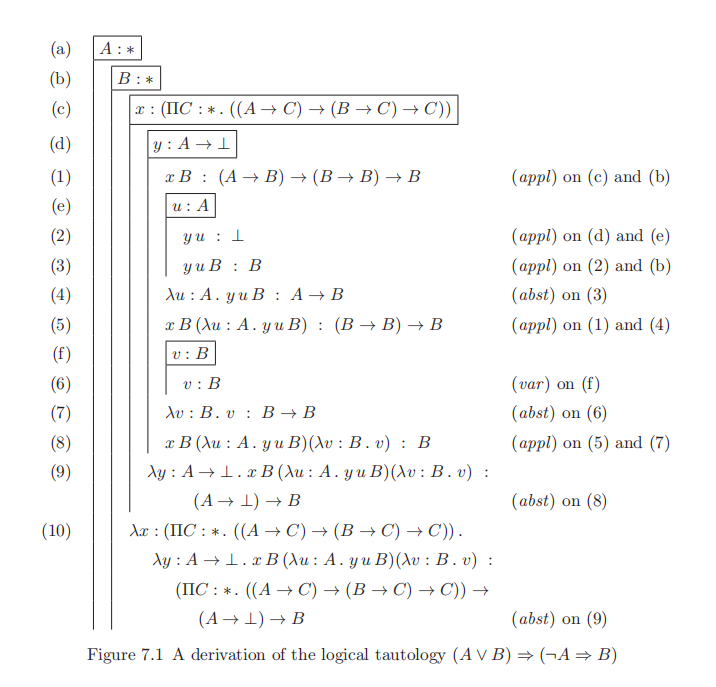
\includegraphics[width=0.93\linewidth]{"../imgs/7-1.png"}
	
	需要注意的是,如$A\rightarrow B$不能直接通过上下文$A:*,B:*$推导出来,是因为没有$\bot$以产生一个类型为$B$的项。
\end{document}
